%!TEX root = ../hbrs-poster.tex
\documentclass[hbrs-poster.tex]{subfiles}
\usepackage{hyperref}
\begin{document}
    \block{Introduction}
    {
        % \begin{wrapfigure}{l}{16cm}
        %     \vspace{-1cm}
        %     \begin{tikzfigure}
        %         
\includegraphics[scale=0.225]{figures/b-it.pdf}
        %     \end{tikzfigure}
        % \end{wrapfigure}
        % Your content here; in this case, the content is wrapped around a figure, but figures should obviously be placed wherever it makes sense
    
        \textbf{Project Overview:}

        Movie genre classification plays a crucial role in content recommendation systems by providing personalized movie suggestions, boosting user engagement. It significantly improves search functionality, allowing for efficient genre-based filtering and accurate search results. 

        This also provides valuable insights into audience preferences and market trends. This information is crucial for content producers and marketers to understand which genres are gaining popularity, which helps in making informed decisions about future content creation and marketing strategies.\\
        % This classification also facilitates content analysis and insights, enabling trend analysis and guiding market research for informed content production and marketing decisions. Additionally, it supports content creation by helping creators align with genre norms and audience expectations, while also aiding in the curation of thematic or genre-specific collections to improve user experience
        
        
        \textbf{Dataset:}
        \begin{itemize}
            \item 42,306 movie plot summaries extracted from IMDB and Wikipedia,
            including 362 different genres, metadata about the actors and the movies. 
            \begin{tikzfigure}
                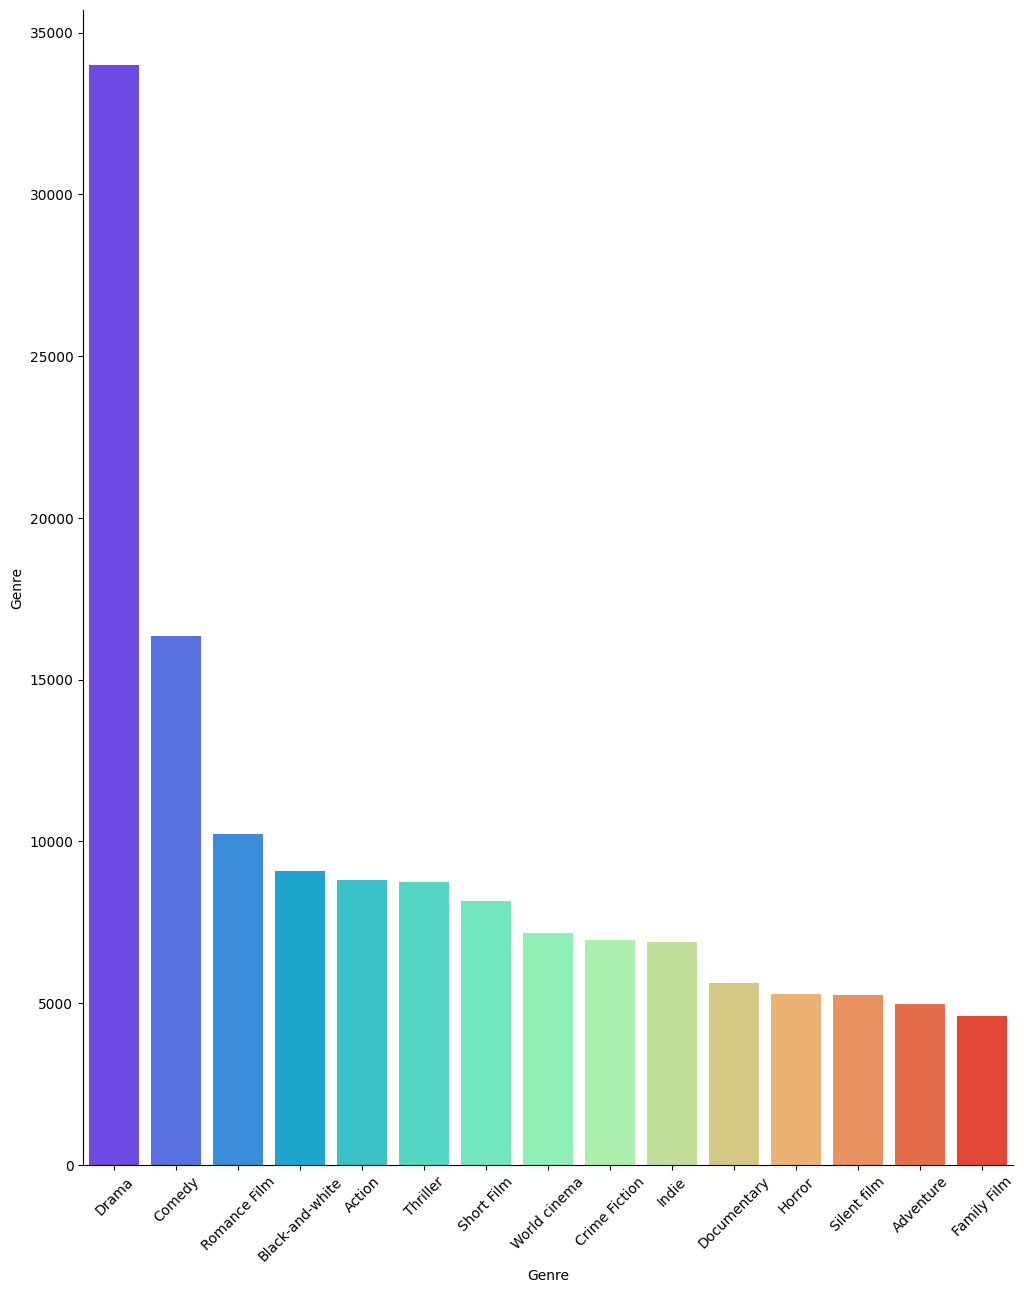
\includegraphics[width=0.325\textwidth, height=0.255\textheight]{figures/output.png}
            \end{tikzfigure}
            \item Due to imbalanced number of labels for each movie genre, we needed to remove few-shot labels, and perform statistical sampling from the original dataset to prevent biased results from trained model.
            \begin{tikzfigure}
                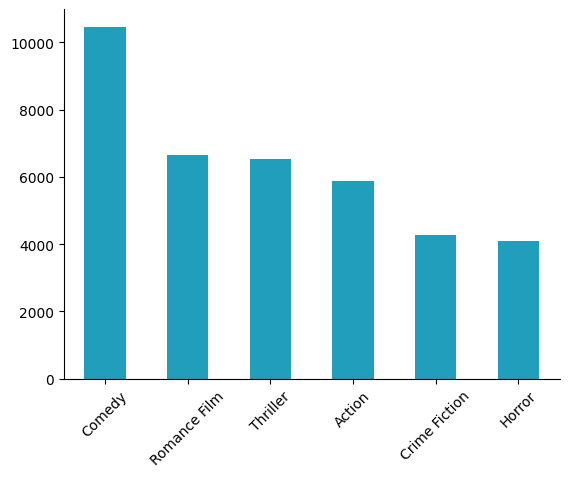
\includegraphics[width=0.325\textwidth, height=0.155\textheight]{figures/output2.png}
            \end{tikzfigure}
        \end{itemize} 
    


    
    }
\end{document}
